%File: formatting-instructions-latex-2024.tex
%release 2024.0
\documentclass[letterpaper]{article} % DO NOT CHANGE THIS
\usepackage{aaai24}  % DO NOT CHANGE THIS
\usepackage{times}  % DO NOT CHANGE THIS
\usepackage{helvet}  % DO NOT CHANGE THIS
\usepackage{courier}  % DO NOT CHANGE THIS
\usepackage[hyphens]{url}  % DO NOT CHANGE THIS
\usepackage{graphicx} % DO NOT CHANGE THIS
\urlstyle{rm} % DO NOT CHANGE THIS
\def\UrlFont{\rm}  % DO NOT CHANGE THIS
\usepackage{natbib}  % DO NOT CHANGE THIS AND DO NOT ADD ANY OPTIONS TO IT
\usepackage{caption} % DO NOT CHANGE THIS AND DO NOT ADD ANY OPTIONS TO IT
\frenchspacing  % DO NOT CHANGE THIS
\setlength{\pdfpagewidth}{8.5in}  % DO NOT CHANGE THIS
\setlength{\pdfpageheight}{11in}  % DO NOT CHANGE THIS
\usepackage{amsmath}
\usepackage{amssymb}
\usepackage{booktabs}
\pdfinfo{
/TemplateVersion (2024.1)
}

\setcounter{secnumdepth}{2}

% Draft notes for the team: resolve and delete before submission.
% To hide all notes at once: \renewcommand{\confirm}[1]{}
\newcommand{\confirm}[1]{\textbf{[#1]}}

\title{Hyperspherical Confidence Mapping for Uncertainty Estimation: Fair Evaluation and Improvements}

\author{
  Ji Qiankun \quad
  Wang Zhongda \quad
  Wei Yutao \\
  Shi Haochen \quad
  Zheng Haoyang
}

\begin{document}
\nocopyright
\maketitle

\begin{abstract}
Hyperspherical Confidence Mapping (HCM) \citep{hcm2026} estimates uncertainty in one forward pass: the network predicts a magnitude and a direction for its target, and the distance of the predicted direction from the unit sphere is the uncertainty score. We reproduce HCM and answer four questions that the paper leaves open. On CIFAR-10 out-of-distribution (OOD) detection with six OOD datasets and five seeds, our runs reach an AUROC of 83.0\% (85.0\% in the paper) and 84.9\% with MixUp (89.4\%); with the same backbone and training, a $k$-nearest-neighbor detector reaches 92.0\%. The five score formulas in the paper and its official code differ only when the predicted magnitude varies. On six UCI regression datasets, we show analytically and empirically that for a scalar target the score measures how uncertain the sign of the target is, so it depends on the origin of the target space and does not rank prediction errors. Two improvements follow. Split conformal calibration with a floored width brings clean-data coverage from 84.5\% to within one point of the nominal 90\%, with intervals about a third as wide. A separate prediction head with HCM applied to the residual brings the error within 0.5\% of a plain network and raises the rank correlation between score and error from 0.15 to 0.24. HCM is a cheap detector of unusual inputs, not a reliable error estimator.
\end{abstract}

\section{Introduction}

A deployed model should report when its prediction is unreliable, but a softmax classifier often assigns high confidence to inputs from outside its training distribution \citep{hendrycks2017baseline}. Existing remedies have costs. Deep ensembles \citep{lakshminarayanan2017simple} and MC Dropout \citep{gal2016dropout} need several forward passes. Evidential methods need one pass but assume a parametric output distribution \citep{sensoy2018evidential,amini2020deep}.

Hyperspherical Confidence Mapping (HCM) \citep{hcm2026} avoids these costs. It writes the target as a magnitude times a unit direction, predicts both with two output heads, and reads uncertainty from how far the predicted direction is from unit length (Figure~\ref{fig:overview}a). It needs one forward pass, no sampling and no distributional assumption, and the same construction covers classification and regression.

\begin{figure}[t]
  \centering
  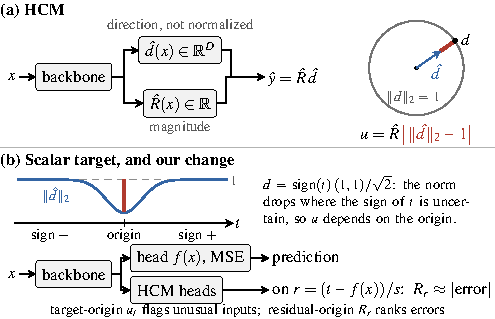
\includegraphics[width=\columnwidth]{fig_overview}
  \caption{(a) HCM decomposes the target into a magnitude and a unit direction and reads uncertainty from the norm of the predicted direction. (b) For a scalar target the direction is only the sign of the target, so the score depends on the origin. We add a prediction head and apply HCM to the residual.}
  \label{fig:overview}
\end{figure}

Reading the paper and its official code, we identify four questions that the paper does not answer. Q2 comes from the code, and the paper's limitations mention Q4 without an experiment.
\textbf{Q1: Is the comparison fair?} The main OOD table does not say whether the baselines were trained with MixUp \citep{zhang2018mixup,thulasidasan2019mixup}, as the best HCM model was, and the paper reports no CIFAR-10 accuracy. In its appendix (Table~8), KNN (93.80\%), MDS (91.31\%) and the ensemble (91.16\%) with MixUp all exceed HCM (90.30\%).
\textbf{Q2: Which score formula?} The paper defines one score, but each of its three official scripts computes a different one.
\textbf{Q3: What does the score measure in regression,} and how can it give intervals with a stated coverage?
\textbf{Q4: How sensitive is training} to the learning rate, the warm-up and the norm penalty?

We reproduce HCM from its official code and answer Q1 in Sections~\ref{sec:cifar-repro} and~\ref{sec:cifar-baselines}, Q2 in Section~\ref{sec:cifar-formulas}, Q3 in Section~\ref{sec:uci}, and Q4 in Sections~\ref{sec:cifar-sensitivity} and~\ref{sec:uci}. Our contributions are:
\begin{itemize}
    \item \textbf{Matched comparison (Q1).} HCM keeps the accuracy of cross-entropy training, but its AUROC is 2.0 to 4.5 points below the paper's and 8 to 9 points below a KNN detector with the same backbone.
    \item \textbf{Ablations (Q2, Q4).} The five score formulas differ only when the predicted magnitude varies. A norm penalty of weight 1 lowers the AUROC by 10.8 points.
    \item \textbf{Analysis (Q3).} For a scalar target the score measures the uncertainty of the sign of the target. It depends on the origin and does not rank errors.
    \item \textbf{Improvements.} Conformal calibration with a floored width gives valid coverage on clean data. A prediction head and a residual-origin HCM remove the accuracy cost and give a score that follows the error (Figure~\ref{fig:overview}b).
\end{itemize}

\section{Related Work}
\label{sec:related}

\paragraph{OOD detection.} Post-hoc detectors score a trained classifier. The maximum softmax probability (MSP) \citep{hendrycks2017baseline}, ODIN \citep{liang2018enhancing} and the energy score \citep{liu2020energy} use the logits; the Mahalanobis distance score (MDS) \citep{lee2018simple} and the $k$-nearest-neighbor (KNN) score \citep{sun2022knn} use distances to training features.

\paragraph{Uncertainty estimation.} Deep ensembles and MC Dropout estimate uncertainty from the spread of several predictions, and evidential networks predict the parameters of a prior distribution in one pass, as do DUQ and SNGP \citep{vanamersfoort2020duq,liu2020sngp}. Split conformal prediction \citep{lei2018conformal,romano2019cqr} turns any score into intervals with finite-sample marginal coverage on exchangeable data. Hyperspherical methods such as ArcFace, CIDER and SIREN \citep{deng2019arcface,ming2023cider,du2022siren} normalize features and class weights so that classification depends on angles. HCM does not normalize features and has no class prototypes: its unit-norm condition applies to the direction of the predicted output, and the violation of that condition is the uncertainty signal.

\section{Background: Hyperspherical Confidence Mapping}
\label{sec:method}

HCM treats classification and regression alike as regression onto a target vector $y\in\mathbb{R}^D$. The target is written as a magnitude times a direction,
\[
  y = R\,d,\qquad R=\lVert y\rVert_2,\qquad \lVert d\rVert_2=1 .
\]
The network has two output heads on a shared backbone: a direction head $\hat d(x)\in\mathbb{R}^D$ and a magnitude head $\hat R(x)\in\mathbb{R}$. Its prediction is $\hat y=\hat R\,\hat d$. For classification with $C$ classes, $y$ is the one-hot label, so $D=C$, $R=1$ and $d=y$, and the predicted class is $\arg\max_c \hat y_c$. For a scalar target $t$, the paper sets $y=(t,t)$.

The true direction always has unit norm, but the direction head is not normalized. HCM uses the violation of this constraint as its uncertainty score (Eq.~2 of the paper):
\begin{equation}
  u(x)=\hat R(x)\,\bigl\lvert\lVert\hat d(x)\rVert_2-1\bigr\rvert .
  \label{eq:score}
\end{equation}
Proposition~1 of the paper bounds the error from below: $\lVert\hat y-y\rVert_2\ge u(x)(1-\epsilon)$ with $\epsilon=\lvert\hat R-R\rvert/(\hat R\,\lVert\hat d-d\rVert_2)$. A large $u$ therefore implies a large error, but a small $u$ does not imply a small error.

The training loss (Eq.~3 of the paper) has a direction term, a magnitude term and a penalty on the norm:
\begin{equation}
\begin{split}
  \mathcal{L}={}&\phi_d\bigl(R\,\lVert\hat d-d\rVert_2\bigr)+\phi_R\bigl(\hat R-R\bigr)\\
  &+\lambda_{\text{norm}}\,\phi_{\text{norm}}\bigl(\bigl\lvert\lVert\hat d\rVert_2-1\bigr\rvert\bigr),
\end{split}
  \label{eq:hcm-loss}
\end{equation}
where each $\phi$ is a loss of the same family (the paper names power, Huber and smooth-$\ell_1$ losses). The paper's experiments use the squared loss. It gives no default for $\lambda_{\text{norm}}$ and recommends starting from 0.

\paragraph{Paper versus official code.} The official repository has three scripts (CIFAR-10, a 1D toy regression and two moons) and no code for MixUp, the UCI experiments or the baselines. Two differences matter below. First, the CIFAR-10 script minimizes $\mathrm{MSE}(\hat d,y)^{3/4}+\mathrm{MSE}(\hat R\,y,y)^{3/4}$ with no norm penalty, and multiplies the loss by 0.1 in the first two epochs. Second, each script computes a different score (Section~\ref{sec:cifar-formulas}).

\section{Image OOD Detection on CIFAR-10}
\label{sec:exp}

\subsection{Setup}
\label{sec:cifar-setup}

\paragraph{Training.} We follow the official CIFAR-10 script: a ResNet-18 for $32\times32$ inputs \citep{he2016deep} with a linear direction head (10 outputs) and a linear magnitude head (1 output), SGD with momentum 0.9, weight decay $10^{-4}$ and batch size 64, 100 epochs, a learning rate of 0.1 divided by 10 at epochs 30, 60 and 90, random crops and horizontal flips. HCM uses the loss of the official script ($\lambda_{\text{norm}}=0$), including its factor of 0.1 in the first two epochs. The cross-entropy (CE) networks use the same backbone, schedule, augmentation and warm-up. We evaluate the last-epoch model.

\paragraph{MixUp.} The paper describes pairwise MixUp ($k=2$) and a Dirichlet variant ($k=20$ samples, weights from $\mathrm{Dir}(0.5)$) without saying which gives its main result. We implement both; pairwise MixUp draws one weight from $\mathrm{Beta}(1,1)$ per batch and mixes every batch. A mixed label $\tilde y$ has a norm below 1, so the HCM targets can be built in two ways. \textbf{Soft} targets set $d^*=\tilde y$ and $R^*=1$, so the direction target is not a unit vector. \textbf{Decomposed} targets set $R^*=\lVert\tilde y\rVert_2$ and $d^*=\tilde y/\lVert\tilde y\rVert_2$, so it stays on the unit sphere.

\paragraph{Evaluation.} CIFAR-10 is the in-distribution (ID) set. The six OOD sets are those named in the OpenOOD CIFAR-10 benchmark \citep{yang2022openood,zhang2023openood}: CIFAR-100 and Tiny ImageNet (TIN) as near-OOD, and MNIST, SVHN, DTD and Places365 as far-OOD. We load them as the official repository does, not from OpenOOD's curated lists. We report AUROC and FPR@95, the fraction of OOD samples accepted as ID at the threshold that keeps 95\% of the ID samples (ID positive, as in the early OpenOOD code; the current OpenOOD code and the official script treat OOD as positive). The paper does not define the metric and neither convention reproduces its FPR values, so we compare FPR@95 only among our own runs. Unless stated otherwise, the HCM score is Eq.~\eqref{eq:score} and results are means over five seeds.

\paragraph{Baselines.} MSP, MDS, KNN and an ensemble of the five seeds all use the CE networks, trained with and without pairwise MixUp.

\subsection{Reproduction and MixUp Variants}
\label{sec:cifar-repro}

\begin{table}[t]
  \centering
  \small
  \setlength{\tabcolsep}{1mm}
  \begin{tabular}{@{}lcccc@{}}
    \toprule
    & & \multicolumn{2}{c}{Pairwise MixUp} & Dirichlet \\
    \cmidrule(lr){3-4}
    & No MixUp & decomposed & soft & MixUp \\
    \midrule
    CE accuracy  & $94.07_{0.08}$ & \multicolumn{2}{c}{$94.85_{0.15}$} & $84.97_{0.44}$ \\
    HCM accuracy & $94.23_{0.18}$ & $94.81_{0.13}$ & $94.65_{0.14}$ & $85.50_{0.40}$ \\
    \midrule
    HCM AUROC &$83.04_{0.29}$ & $\mathbf{84.90}_{1.27}$ & $81.72_{2.63}$ & $77.44_{1.16}$ \\
    \quad CIFAR-100 & $80.6_{0.4}$ & $83.4_{0.7}$ & $84.0_{1.4}$ & $79.3_{0.6}$ \\
    \quad TIN       & $81.7_{0.6}$ & $84.2_{0.8}$ & $85.7_{1.2}$ & $80.9_{0.6}$ \\
    \quad MNIST     & $84.3_{0.7}$ & $89.4_{3.4}$ & $71.4_{7.8}$ & $76.9_{8.7}$ \\
    \quad SVHN      & $83.6_{1.1}$ & $81.6_{6.3}$ & $80.2_{11.1}$ & $70.0_{2.3}$ \\
    \quad DTD       & $85.6_{0.4}$ & $88.0_{2.1}$ & $83.8_{3.0}$ & $79.4_{0.8}$ \\
    \quad Places365 & $82.4_{0.6}$ & $82.8_{0.5}$ & $85.1_{1.4}$ & $78.3_{0.9}$ \\
    \midrule
    HCM FPR@95 &$59.94_{1.76}$ & $49.88_{2.17}$ & $56.71_{2.65}$ & $80.14_{2.40}$ \\
    \bottomrule
  \end{tabular}
  \caption{CIFAR-10 accuracy and OOD detection of HCM in \%. HCM AUROC and FPR@95 are averages over the six OOD sets; the indented rows give the AUROC per set. Subscripts are standard deviations over five seeds (three for Dirichlet MixUp). The paper reports an AUROC of 85.04 without and 89.44 with MixUp.}
  \label{tab:hcm_overall}
\end{table}

\paragraph{HCM keeps the accuracy of CE (Q1).} Table~\ref{tab:hcm_overall} shows $94.23\%$ for HCM against $94.07\%$ for CE, and $94.81\%$ against $94.85\%$ with pairwise MixUp. MixUp raises accuracy by 0.4 to 0.8 points for both. The paper does not report accuracy.

\paragraph{The reproduced AUROC is below the paper's.} We obtain $83.04\%$ against $85.04\%$ without MixUp, and $84.90\%$ against $89.44\%$ with pairwise MixUp and decomposed targets. MixUp helps by 1.9 points instead of 4.4. The likely sources are details that the paper leaves open (the MixUp variant, the score formula, $\lambda_{\text{norm}}$, the warm-up and the checkpoint selection) and the OOD splits.

\paragraph{The target construction matters.} Soft targets are 3.2 points below decomposed targets and below HCM without MixUp. Both raise the near-OOD AUROC by 2.5 to 4.0 points but differ on far-OOD data. Soft targets lower MNIST by 12.9 points. Decomposed targets raise MNIST by 5.1 and DTD by 2.4 points but lower SVHN by 2.0 points, where the standard deviation over seeds is 6.3 points. We chose decomposed targets as the main setting after seeing these results, so we report both. Dirichlet MixUp lowers accuracy by about 9 points for CE as well as for HCM, which points to the augmentation and not to HCM, and we do not use it below.

\subsection{Comparison with Baselines}
\label{sec:cifar-baselines}

\begin{figure}[t]
  \centering
  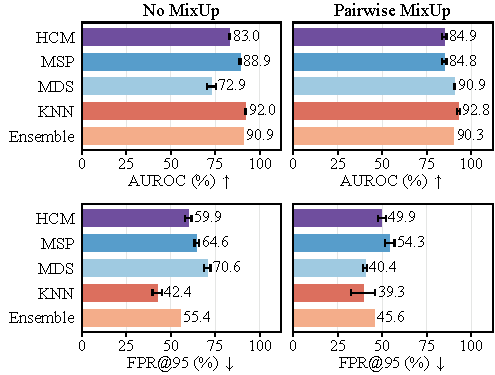
\includegraphics[width=\linewidth]{fig_fair_comparison}
  \caption{OOD detection under matched training, without MixUp (left) and with pairwise MixUp (right), averaged over six OOD sets. Bars are five-seed means with standard deviations; the ensemble combines the five seeds.}
  \label{fig:fair}
\end{figure}

Figure~\ref{fig:fair} completes the answer to Q1: all methods share the training setting.

\paragraph{Without MixUp.} KNN is the best detector (AUROC $92.01\pm0.36\%$, FPR@95 $42.36\pm2.62\%$), followed by the ensemble ($90.90\%$) and MSP ($88.93\pm0.31\%$). HCM ($83.04\pm0.29\%$) is 6 to 9 points below these three in AUROC, but its FPR@95 ($59.9\%$) is lower than that of MSP ($64.6\%$) and MDS ($70.6\%$).

\paragraph{With pairwise MixUp.} KNN ($92.75\pm0.85\%$), MDS ($90.87\pm0.23\%$) and the ensemble ($90.33\%$) are 5 to 8 points above HCM with decomposed targets ($84.90\pm1.27\%$). MSP falls by 4.1 points to $84.82\pm1.29\%$ and is level with HCM in AUROC; HCM has the lower FPR@95 ($49.9\%$ against $54.3\%$).

\paragraph{Baseline strength.} Our MSP, KNN and ensemble results without MixUp are 0.8 to 1.1 points above the values in the HCM paper ($87.85\%$, $90.97\%$, $90.15\%$), so these baselines are not weakened. MDS is the exception: without MixUp it reaches $72.90\pm2.38\%$ against $89.34\%$ in the paper. Changing the ridge regularization of the covariance does not close this gap, so this result should be read with caution; the conclusion that KNN exceeds HCM does not depend on it.

\subsection{Score Formulas}
\label{sec:cifar-formulas}

\begin{table}[t]
  \centering
  \small
  \setlength{\tabcolsep}{1mm}
  \begin{tabular}{@{}llcc@{}}
    \toprule
    Name & Score & AUROC & FPR@95 \\
    \midrule
    Eq.~\eqref{eq:score} (paper) & $\hat R\,\lvert n-1\rvert$ & $84.90_{1.27}$ & $49.88_{2.17}$ \\
    Norm only  &$\lvert n-1\rvert$ & $84.54_{1.28}$ & $51.03_{2.24}$ \\
    CIFAR-10 script     & $\max(n,1/n)-1$ & $84.48_{1.29}$ & $51.04_{2.23}$ \\
    Toy script          & $\hat R\sqrt{\lvert n^2-1\rvert}$ & $\mathbf{85.22}_{1.23}$ & $\mathbf{48.68}_{1.94}$ \\
    Two-moons script    & $\lvert\hat R\,n-1\rvert$ & $80.30_{1.30}$ & $56.36_{2.29}$ \\
    \bottomrule
  \end{tabular}
  \caption{The five score formulas, with $n=\lVert\hat d\rVert_2$, and their six-dataset results in \% for HCM with pairwise MixUp and decomposed targets (five seeds). Monotone transformations in the scripts, which do not change the metrics, are omitted.}
  \label{tab:score_formulas}
\end{table}

This section answers Q2. The paper defines the score of Eq.~\eqref{eq:score}. Each official script computes a different one, and the README gives a fourth form for classification (Table~\ref{tab:score_formulas}). We evaluate all five on the same trained networks, without retraining.

Without MixUp and with soft targets, the five formulas agree within 0.04 points in every metric (AUROC $83.02$--$83.04\%$ and $81.70$--$81.74\%$): the magnitude target is always 1, so $\hat R$ stays at 1.000 on the test set. With decomposed targets the magnitude follows the norm of the mixed label (mean test $\hat R=0.854$), and the choice matters. The two-moons formula is 4.6 points below Eq.~\eqref{eq:score}, mainly because of MNIST ($66.53\%$). The other four differ by less than one standard deviation over seeds, but their order (toy script, Eq.~\eqref{eq:score}, norm only, CIFAR-10 script) is the same in each of the five seeds.

\subsection{Training Sensitivity}
\label{sec:cifar-sensitivity}

\begin{table}[t]
  \centering
  \small
  \setlength{\tabcolsep}{1.5mm}
  \begin{tabular}{@{}lccc@{}}
    \toprule
    Setting & Acc. & AUROC & FPR@95 \\
    \midrule
    Baseline & 94.60 & 83.32 & 51.76 \\
    Learning rate 0.05 & 94.52 & 85.30 & 54.73 \\
    Learning rate 0.2 & 95.26 & 87.44 & 44.68 \\
    Warm-up 5 epochs & 94.77 & 87.23 & 47.64 \\
    No warm-up & 94.36 & 85.99 & 49.42 \\
    $\lambda_{\text{norm}}=0.1$ & 94.50 & 81.13 & 56.39 \\
    $\lambda_{\text{norm}}=1.0$ & 94.53 & 72.52 & 68.03 \\
    Loss power 1 & 95.10 & 82.85 & 60.17 \\
    Soft MixUp targets & 94.49 & 81.86 & 57.24 \\
    Paper-form loss & \multicolumn{3}{c}{diverged} \\
    \bottomrule
  \end{tabular}
  \caption{Sensitivity of HCM on CIFAR-10 in \% (seed 0, last checkpoint, averages over six OOD sets). One setting is changed at a time.}
  \label{tab:sensitivity}
\end{table}

This section answers Q4 for the image task, for which the paper reports no sensitivity analysis. We change one setting at a time around a baseline: HCM with pairwise MixUp and decomposed targets, trained as in Section~\ref{sec:cifar-setup}. Each run uses seed 0; the seed-to-seed standard deviation of this configuration is 1.27 points of AUROC and 2.17 points of FPR@95.

Table~\ref{tab:sensitivity} shows three patterns. First, the norm penalty harms OOD detection: $\lambda_{\text{norm}}=1$ costs 10.8 points of AUROC and 16.3 points of FPR@95 at unchanged accuracy, far beyond the seed variation. Second, the learning rate and the warm-up change the AUROC by 2 to 4 points, but not monotonically: halving and doubling the learning rate both raise it, as do a longer warm-up and no warm-up, so one seed cannot separate these effects from noise. Third, removing the exponent $3/4$ and using soft targets raise FPR@95 by 8.4 and 5.5 points. The run with the loss in the form of Eq.~\eqref{eq:hcm-loss} diverged.

% Scalar regression on UCI datasets. \input this file from the main report.
% It needs amsmath, amssymb, graphicx, booktabs; the figures sit next to the .tex files.
% It refers to eq:score and eq:hcm-loss, which are defined in the main file.

\section{Scalar Regression on UCI Datasets}
\label{sec:uci}

This section answers Q3 (what the score measures for a scalar target, and how to obtain
intervals with a stated coverage) and the regression part of Q4 (training sensitivity). The
HCM paper evaluates regression on six UCI datasets \citep{dua2017uci,hernandez2015pbp} and reports one
result: the score $u$ grows when Gaussian noise is added to the test inputs. The official
repository has no UCI code, so the implementation is ours.

\subsection{Setup}
\label{sec:uci-setup}

We use the paper's six datasets (wine, concrete, energy, kin8nm, power, yacht) and its
protocol (Appendix~A.1): a random 80/10/10 split, an MLP with three hidden layers of 20
units, Adam with weight decay $10^{-4}$, 200 epochs, and test inputs perturbed by
$\mathcal{N}(0,\sigma^2 I)$ with $\sigma\in\{0,\dots,5\}$. The paper does not state the
batch size or the input scaling; we use batch size 64 and standardized inputs. The baselines share the trunk: a plain MLP, a Deep Ensemble of five
Gaussian-likelihood networks \citep{lakshminarayanan2017simple}, and MC Dropout with rate
0.1 and 50 passes \citep{gal2016dropout}. Results are means over 20 seeds (5 for sweeps).

Following Section~2.2 of the paper, a scalar target $t$ is embedded as $y=(t,t)$, so that
\begin{equation}
  R=\lVert y\rVert_2=\sqrt{2}\,\lvert t\rvert,\qquad
  d=\frac{y}{R}=\operatorname{sign}(t)\,\frac{(1,1)}{\sqrt{2}} .
  \label{eq:scalar}
\end{equation}
The network has a direction head $\hat d\in\mathbb{R}^2$ and a magnitude head
$\hat R\in\mathbb{R}$ and minimizes
\begin{equation}
  \mathcal{L}=\operatorname{MSE}(\hat R\,d,\;y)+\operatorname{MSE}(R\,\hat d,\;y)
  +\lambda_{\text{norm}}\bigl(\lVert\hat d\rVert_2-1\bigr)^2 ,
  \label{eq:loss}
\end{equation}
the squared-loss instance of Eq.~\eqref{eq:hcm-loss}, with $\lambda_{\text{norm}}=0$ unless
stated, as the paper recommends. The prediction is the mean of the two components of
$\hat R\hat d$ (the paper does not specify this). The score is Eq.~\eqref{eq:score} with
$\lvert\hat R\rvert$ in place of $\hat R$, because the magnitude head is an unconstrained
linear output.

\subsection{Reproduction and the learning rate}
\label{sec:uci-lr}

With the paper's stated setting (raw targets, learning rate $10^{-4}$), HCM does not finish
training on three datasets: its test RMSE is $1.67$, $1.69$ and $1.17$ times the standard
deviation of the targets on concrete, energy and yacht, worse than predicting the training
mean. The unstated batch size explains part of the gap to the paper: with batch size 1 our
validation MAE on concrete falls from $22.2$ to $4.94$ (paper: $4.31$). We therefore train
every method, including the baselines, with standardized targets and learning rate
$10^{-3}$, so that no method is undertrained. The RMSE of HCM is then still above that of
the plain MLP on all six datasets, by 2\% (power, wine) to 68\% (energy) (Wilcoxon
signed-rank test over seeds, $p\le 0.017$ on each).

\subsection{What the score measures for a scalar target}
\label{sec:uci-measure}

Eq.~\eqref{eq:scalar} shows that the direction carries one bit: the sign of $t$. With
$\lambda_{\text{norm}}=0$, the two squared-error terms of Eq.~\eqref{eq:loss} are minimized
pointwise by $\hat R^\star(x)=\mathbb{E}[R\mid x]$ and
$\hat d^\star(x)=\mathbb{E}[R^2 d\mid x]\,/\,\mathbb{E}[R^2\mid x]$, hence
\begin{equation}
\begin{split}
\lVert\hat d^\star(x)\rVert_2
&=\frac{\bigl\lvert\mathbb{E}\bigl[t\,\lvert t\rvert \mid x\bigr]\bigr\rvert}
        {\mathbb{E}\bigl[t^2\mid x\bigr]}\;\le\;1, \\
u^\star(x)
&=\sqrt{2}\;\mathbb{E}\bigl[\lvert t\rvert\mid x\bigr]
  \bigl(1-\lVert\hat d^\star(x)\rVert_2\bigr).
\end{split}
\label{eq:ustar}
\end{equation}
The norm equals 1 exactly when the sign of $t$ is certain given $x$. Three predictions
follow, and the experiments confirm each.

\begin{figure}[t]
  \centering
  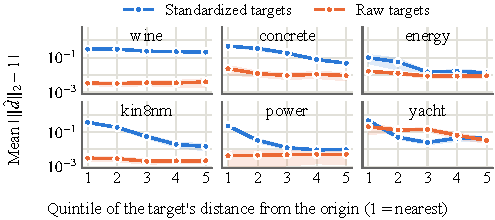
\includegraphics[width=\linewidth]{fig_origin}
  \caption{Violation of the unit-norm constraint by quintile of the target's distance from
  the origin (band: $\pm1$ std over 5 seeds). With standardized targets the violation is
  concentrated near the origin, which is the training mean.}
  \label{fig:origin}
\end{figure}

\emph{(i) With targets of one sign, $u$ carries no information on clean data.} All six raw
UCI targets are positive, so $d$ is constant and $u^\star=0$. In agreement, the mean
$\lVert\hat d\rVert_2$ with raw targets is within $0.015$ of 1 on five datasets.

\emph{(ii) After centering, $u$ marks targets near the mean, not large errors.}
Standardizing makes the sign uncertain near zero. The mean norm drops to between $0.78$ and
$0.98$, and the violation is 10 to 27 times larger in the quintile of targets nearest the
origin than in the farthest one on concrete, kin8nm and power (Figure~\ref{fig:origin}).
The score does not rank errors: on wine, kin8nm and power its Spearman correlation with the
absolute error is at most $0.06$ in absolute value.

\emph{(iii) The HCM prediction is not the conditional mean.} For
$t\mid x\sim\mathcal{N}(\mu,s^2)$ with $\lvert\mu\rvert\ll s$ the prediction is $(4/\pi)\mu$,
a 27\% overshoot, which is consistent with the accuracy cost of
Section~\ref{sec:uci-lr}.

\paragraph{Scale and noisy inputs.} Eq.~\eqref{eq:ustar} is equivariant to rescaling $t$,
but training at a fixed learning rate is not: multiplying the kin8nm target by $0.1$ lowers
the AUROC for detecting noisy inputs ($\sigma=5$) from $0.97$ to $0.35$. The paper's claim
about perturbed inputs does reproduce: with standardized targets the AUROC is $0.86$ to
$0.99$ at $\sigma=5$. The score detects unusual inputs; it does not predict the error.

\subsection{From scores to calibrated intervals}
\label{sec:uci-intervals}

The paper calibrates $u$ with one temperature $T$, fitted so that the coverage of
$\hat y\pm kTu$ for $k=1,2,3$ is closest to $68/95/99.7\%$. This gives no guarantee, and
the paper's own depth-estimation results miss the two higher levels ($0.88$ and $0.92$
against $0.95$ and $0.997$; its Table~3). We replace it with split conformal prediction
\citep{vovk2005algorithmic,angelopoulos2021gentle}. For a nominal coverage $p$ and a width
function $s(x)>0$, the interval is $\hat y(x)\pm q\,s(x)$, where $q$ is the
$\lceil (n+1)p\rceil$-th smallest value of $\lvert y_i-\hat y_i\rvert/s(x_i)$ over the $n$
validation points. Coverage is at least $p$ on exchangeable test data for any $s$. We
compare three width functions for HCM: \textbf{constant}, $s(x)=1$; \textbf{scaled},
$s(x)=u(x)$, the analogue of the paper's rule; and \textbf{floored} (ours),
$s(x)=\max\bigl(1,\,u(x)/u_{95}\bigr)$, where $u_{95}$ is the 95th percentile of $u$ on the
training set. The floored interval keeps a constant width in the usual range of $u$, where
$u$ does not rank errors, and widens only when $u$ is unusually large. IS denotes the
interval score of \citet{gneiting2007strictly}.

\begin{table}[t]
  \centering
  \small
  \setlength{\tabcolsep}{1mm}
  \begin{tabular}{@{}lcccccc@{}}
    \toprule
    & \multicolumn{3}{c}{clean test} & \multicolumn{2}{c}{$\sigma=1$} & $\sigma=5$ \\
    \cmidrule(lr){2-4}\cmidrule(lr){5-6}\cmidrule(l){7-7}
    Method & cov. & width & IS & cov. & IS & IS \\
    \midrule
    HCM temp.\ (paper)         & 0.845 & 2.87 & 3.46 & 0.752 & 15.8 & 256 \\
    HCM constant               & 0.896 & 1.01 & 1.40 & 0.359 & 16.6 & 217 \\
    HCM scaled by $u$          & 0.902 & 4.46 & 4.85 & 0.828 & 22.5 & 417 \\
    \textbf{HCM floored (ours)} & \textbf{0.893} & \textbf{1.01} & \textbf{1.39} & \textbf{0.485} & \textbf{10.2} & \textbf{56.0} \\
    \midrule
    MCD Gaussian               & 0.704 & 0.59 & 2.30 & 0.367 & 10.1 & 38.3 \\
    MCD conformal              & 0.900 & 1.16 & 1.49 & 0.539 & 7.8  & 30.9 \\
    DE Gaussian                & 0.925 & 0.91 & 1.18 & 0.456 & 9.9  & 42.3 \\
    DE conformal               & 0.905 & 0.89 & 1.18 & 0.427 & 10.3 & 42.6 \\
    \bottomrule
  \end{tabular}
  \caption{Prediction intervals at nominal coverage $0.90$ (six datasets, 20 seeds). Width
  and interval score (IS, lower is better) are in units of std($y$). Temp.\ is the paper's
  temperature rule; constant, scaled and floored are conformal. MCD: MC Dropout; DE: Deep
  Ensemble.}
  \label{tab:intervals}
\end{table}

Table~\ref{tab:intervals} supports four conclusions.
\emph{(1) Conformal calibration repairs the paper's under-coverage.} The temperature rule
covers $84.5\%$ at a nominal $90\%$. Every conformal variant is within about one point of
$90\%$ on clean data, and the constant and floored intervals are about a third as wide.
\emph{(2) Scaling the width by $u$ is harmful.} Because $u$ is close to zero for many clean
inputs, the intervals are $4.4$ times wider.
\emph{(3) The floored rule keeps the benefit of $u$ without that cost.} On clean data it
matches the constant interval ($1.39$ against $1.40$). Under input noise it lowers the
interval score from $16.6$ to $10.2$ at $\sigma=1$ and from $217$ to $56$ at $\sigma=5$.
\emph{(4) HCM does not beat the sampling baselines, but it is cheaper.} The Deep Ensemble
has the best clean interval score ($1.18$). At $\sigma=1$ floored HCM equals it ($10.2$
against $10.3$) with one network instead of five; at $\sigma=5$ it is behind both
baselines. Under noise no method keeps the guarantee: coverage at $\sigma=1$ falls to
between $0.36$ and $0.54$, except for the two very wide HCM intervals.

\subsection{Our Improvements: a Prediction Head and Residual-Origin HCM}
\label{sec:uci-fix}

Section~\ref{sec:uci-measure} found two causes of the problems above: the HCM prediction is
not the conditional mean, and the origin of the decomposition is arbitrary. Each suggests
one change; both keep the loss of Eq.~\eqref{eq:loss}.

\paragraph{A separate prediction head.} We add a linear head $f(x)$ trained with the plain
MSE and use it as the prediction; the HCM heads only produce the score. When the HCM heads
are \emph{detached} (they read the trunk features but send no gradient back) or have their
\emph{own} trunk, the accuracy cost disappears: the test RMSE is $1.003$ and $1.005$ times
that of the plain MLP (Wilcoxon, $p\ge 0.097$ on every dataset). With a shared trunk the
ratio is $1.09$ (Figure~\ref{fig:fix}, top left).

\paragraph{Residual-origin HCM.} We apply the decomposition to the standardized residual
$r=(t-f(x))/s$ instead of the target, where $s$ is a running root-mean-square of the
training residuals and no gradient flows into $f$. Eq.~\eqref{eq:ustar} holds with $r$ in place of $t$: if the sign of the residual
cannot be predicted from $x$, then $\lVert\hat d^\star\rVert_2=0$ and
$\hat R^\star=\sqrt2\,\mathbb{E}[\lvert r\rvert\mid x]$, the expected absolute error up to a
constant. We therefore use $R_r=s\,\lvert\hat R\rvert$ as the score.

On clean data the new score does what $u$ could not (Table~\ref{tab:fix}). Its Spearman
correlation with the absolute error is $0.24$ against $0.15$ for $u$. A conformal interval
with width proportional to $R_r$ has an interval score of $1.27$, against $1.39$ for
floored HCM. The cost is that $R_r$ does not
detect unusual inputs: its AUROC at $\sigma=5$ is $0.67$ against $0.94$ for $u$. The two
scores are complementary: $R_r$ ranks errors on data like the training data, and the
target-origin score, written $u_t$, flags inputs unlike it.

\begin{table}[t]
  \centering
  \small
  \setlength{\tabcolsep}{1mm}
  \begin{tabular}{@{}lcccccc@{}}
    \toprule
    & & & & clean & $\sigma=1$ & $\sigma=5$ \\
    Width function & RMSE & $\rho$ & AUROC & IS & IS & IS \\
    \midrule
    HCM, floored $u$           & 1.196 & 0.15 & 0.94 & 1.39 & 10.2 & 56.0 \\
    \midrule
    \multicolumn{7}{@{}l}{\emph{Prediction head, detached HCM heads (one trunk)}} \\
    floored $u_t$              & 1.003 & 0.13 & 0.86 & 1.32 & 11.7 & 43.1 \\
    $R_r$                      & 1.003 & 0.24 & 0.67 & 1.27 & 13.7 & 74.0 \\
    both, product rule         & 1.003 & 0.24 & 0.84 & 1.27 & 11.5 & 63.9 \\
    \textbf{both, max rule}    & \textbf{1.003} & \textbf{0.23} & \textbf{0.89} & \textbf{1.27} & \textbf{11.8} & \textbf{43.5} \\
    \midrule
    \multicolumn{7}{@{}l}{\emph{Prediction head, HCM heads with their own trunks}} \\
    both, max rule             & 1.005 & 0.28 & 0.94 & 1.27 & 10.7 & 50.2 \\
    \midrule
    Deep Ensemble              & 1.244 & 0.42 & 0.98 & 1.18 & 10.2 & 42.6 \\
    MC Dropout                 & 1.431 & 0.15 & 0.97 & 1.49 & 7.8  & 30.9 \\
    \bottomrule
  \end{tabular}
  \caption{Our improvements (six datasets, 20 seeds, conformal intervals at nominal coverage
  $0.90$; clean coverage $0.893$ to $0.905$). RMSE is relative to the plain MLP; $\rho$ is
  the Spearman correlation of the width with the absolute error; AUROC is for noisy inputs
  at $\sigma=5$. Bold: our proposed variant.}
  \label{tab:fix}
\end{table}

\begin{figure}[t]
  \centering
  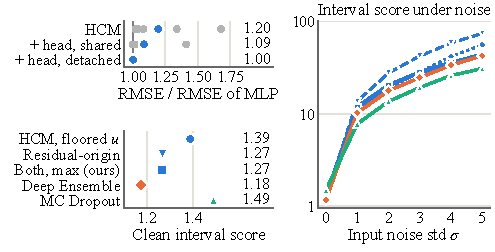
\includegraphics[width=\linewidth]{fig_changes}
  \caption{Top left: test RMSE relative to the plain MLP (gray: single datasets).
  Bottom left: clean interval score. Right: interval score under input noise (same
  markers). Six datasets, 20 seeds, detached heads.}
  \label{fig:fix}
\end{figure}

\paragraph{Using both scores.} With detached heads, a target-origin pair and a
residual-origin pair can share one trunk and one forward pass. We compare two width functions, with $u_{95}$ as in
Section~\ref{sec:uci-intervals} and $\bar R_r$ the training mean of $R_r$:
\begin{align*}
\text{product:}\quad s(x) &= R_r(x)\,\max\!\Bigl(1,\frac{u_t(x)}{u_{95}}\Bigr),\\
\text{max:}\quad s(x) &= \max\!\Bigl(\frac{R_r(x)}{\bar R_r},\,\frac{u_t(x)}{u_{95}}\Bigr).
\end{align*}
Both keep the clean-data gain ($1.27$). The product rule fails at $\sigma=5$ ($63.9$). The
max rule reaches $43.5$ at $\sigma=5$, better than floored HCM ($56.0$) and level with the
Deep Ensemble ($42.6$), but at $\sigma=1$ it is worse than floored HCM ($11.8$ against
$10.2$). Over five target preprocessings the interval score of $R_r$ ranges from $1.29$ to
$1.75$, against $3.57$ to $6.79$ for the original score. Residual-origin HCM is close to estimating the absolute residual for locally weighted
conformal intervals \citep{lei2018conformal}.

\paragraph{Norm penalty and warm-up (Q4).} With standardized targets, raising
$\lambda_{\text{norm}}$ from 0 to 5 moves the mean norm from $0.88$ to $0.99$, raises the
test error on 26 of 30 dataset--seed pairs, and raises the AUROC for noisy inputs from
$0.93$ to $0.97$ at $\sigma=5$. A warm-up of 5 or 20 epochs changes the normalized RMSE by
at most $0.01$ and the AUROC by at most $0.02$, so it is not needed here.

\paragraph{Limitations.}
\label{sec:uci-limits}
The network is a small MLP. The analysis assumes squared losses,
$\lambda_{\text{norm}}=0$ and clean inputs, so it does not explain why $u$ rises under
noise. The max rule was selected on the noisy test sets, so its results under noise are exploratory.


\section{Discussion and Conclusion}
\label{sec:conclusion}

\paragraph{What matched our expectation.} The cost claims of HCM hold: one forward pass, no sampling, and no loss of classification accuracy. Both improvements work: conformal calibration with a floored width repairs the under-coverage, and a prediction head with HCM on the residual removes the accuracy cost. The two scores are complementary: the residual-origin score ranks errors, the target-origin score flags unusual inputs.

\paragraph{What we found beyond the paper.} Q1: our AUROC is 2.0 to 4.5 points below the paper's, and under matched training HCM is 8 to 9 points below KNN. Q2: the paper and its code disagree on the score, which matters only when the magnitude varies. Q3: the regression score is not an error estimate; it measures the uncertainty of the sign of the target relative to a chosen origin. Q4: the norm penalty acts differently by task: $\lambda_{\text{norm}}=1$ costs 10.8 AUROC points on CIFAR-10 (one seed), while on UCI raising it from 0 to 5 raises both the AUROC for noisy inputs (0.93 to 0.97) and the test error.

\paragraph{Conclusion.} HCM is a cheap detector of unusual inputs, not a reliable error estimator, and in regression it needs conformal calibration and the residual origin to be useful.

\paragraph{Limitations.} The CIFAR-10 sensitivity results use one seed, and the gap to the paper's AUROC and the low MDS result without MixUp remain unexplained. The regression study uses a small MLP, and its max rule was selected on test results (Section~\ref{sec:uci-limits}).

\bibliography{aaai24}

\end{document}
